% Copyright Patrick Hall 2019
% CC by 4.0 license
% TODO: 
% - DIA on single DT instead

\documentclass[fleqn]{article}

\renewcommand\refname{}

\title{Guidelines for Responsible and Human-Centered Use of Explainable Machine Learning}

\author{
  \copyright \hspace{1pt} Patrick Hall 2019\footnote{H2O.ai and George Washington University}, \\
  Washington, DC\\
  \texttt{patrick.hall@h2o.ai}
}

\usepackage{graphicx}
\usepackage{fullpage}
\usepackage{pdfpages}
\usepackage{amsmath}
\usepackage{amssymb}
\usepackage{mathtools}
\usepackage{MnSymbol}
\usepackage{enumerate}
\usepackage{setspace}
\usepackage[hyphens]{url}
\usepackage[colorlinks]{hyperref}
\usepackage{float}
\usepackage{caption}
\usepackage{subcaption}
\usepackage{multicol}
\usepackage{color}
\usepackage{listings}
\usepackage{csvsimple}
\usepackage{algorithm}
\usepackage{algorithmic}
\usepackage{verbatim}
\usepackage{mdframed}
\usepackage{changepage}
\usepackage[top=1in, bottom=1in, left=1in, right=1in]{geometry}

%two part definition
\newcommand{\twopartdef}[4]
{
	\left\{
		\begin{array}{ll}
			#1 & \mbox{if } #2 \\
			#3 & \mbox{if } #4
		\end{array}
	\right.
}

\begin{document}

\maketitle

\section*{Introduction}

%Due to obvious community and commercial demand, explainable machine learning (ML) methods have already been implemented in popular open source software and in commercial software.\footnote{Like H2O-3, XGBoost, and various other Python and R packages. See: \url{https://github.com/jphall663/awesome-machine-learning-interpretability} for a longer, curated list of relevant open source software packages.}\textsuperscript{,}\footnote{For instance  Datarobot, H2O Driverless AI, SAS Visual Data Mining and Machine Learning, Zest AutoML, and likely several others.} Yet, as someone who has been involved in the implementation of explainable ML software for the past three years, I find a lot of what I read about the topic confusing and detached from my personal, hands-on experiences. This short opinion paper presents arguments, proposals, and references to address some observed explainable ML misconceptions. Please note that this text is not an attack on any party, and disagreements with any previous credible opinion pieces are mostly minor and technical.\footnote{For instance, say ``Please Stop Explaining Black Box Models for High Stakes Decisions'' \cite{please_stop}.} This text is instead a call for pragmatism from the trenches. It seeks to promote nuanced debate, responsible use, and continued development of explainable ML, and not dismissal or derision of the discipline.  Moreover, this text builds the seemingly natural case for a holistic approach to ML that includes interpretable (i.e. ``white-box'') models along with explanatory, debugging, and disparate impact analysis techniques.\\

%``Please stop doing explainable machine learning,'' extolled one of the brightest minds in machine learning (ML) with the title of a recent and well-reasoned essay \cite{please_stop}. A related and admittedly-controversial short talk also included points such as, ``[Explainable ML] forces you to rely on two models instead of one,'' and argued that explainable machine learning can be a foil for companies and governments to conduct unsavory or negligent deeds with black-box models.\footnote{Statistics at a Crossroads, Webinar 2. URL: \url{https://zoom.us/recording/play/0y-iI9HamgyDzzP2k_jiTu6jB7JgVVXnjWZKDMbnyRTn3FsxTDZy6Wkrj3_ekx4J?startTime=1538497702000}} Perhaps even more noteworthy was the online response, which included musings such as, ``don’t forget hidden assumptions for explainable ML (e.g., locally linear behavior near predictions),'' and lamentations like, ``no one has explained to me what 'explainable' or 'interpretable' is.'' \footnote{Twitter thread: \url{https://twitter.com/tdietterich/status/1052680788389507073}} This article aims to clear up such misconceptions and fill the gaps in community knowledge exposed by these sentiments. Strangely, neither the talk nor the follow-up discussions seemed to allow for combining white-box models and post-hoc explanatory techniques. 

%\begin{figure}[htb]
%	\begin{center}
%		\includegraphics[scale=0.33]{img/figure_1.png}
%		\caption{An augmented learning problem diagram in which several post-hoc techniques create explanations for a credit scoring model $g$. When used properly, explanations can increase understanding of $g$ and help improve the accuracy, fairness, interpretability, privacy, or security of subsequent applications of $\mathcal{H}$ and $\mathcal{A}$. Adapted from Figure 1.2 of the open textbook \textit{Learning From Data} \cite{lfd}.}
%		\label{fig:learning_problem}
%	\end{center}
%\end{figure}	

Explainable machine learning (ML) enables human learning from ML, human appeal of automated model decisions, regulatory compliance, and white-hat hacking and forensic analysis of ML models.\footnote{In the U.S., explanations and the model documentation they enable may be required under the Civil Rights Acts of 1964 and 1991, the Americans with Disabilities Act, the Genetic Information Nondiscrimination Act, the Health Insurance Portability and Accountability Act, the Equal Credit Opportunity Act, the Fair Credit Reporting Act, the Fair Housing Act, Federal Reserve SR 11-7, and the European Union (EU) Greater Data Privacy Regulation (GDPR) Article 22 \cite{ff_interpretability}.}\textsuperscript{,}\footnote{For security applications, see for instance: \url{https://www.oreilly.com/ideas/proposals-for-model-vulnerability-and-security}} XAI techniques have been implemented in numerous open source and commercial packages and XAI is also an important, mandatory, or embedded aspect of commercial predictive modeling in industries like financial services.\footnote{Like H2O-3, XGBoost, and various other Python and R packages. See: \url{https://github.com/jphall663/awesome-machine-learning-interpretability} for a longer, curated list of relevant open source software packages.}\textsuperscript{,}\footnote{For instance  Datarobot, H2O Driverless AI, SAS Visual Data Mining and Machine Learning, Zest AutoML, and likely several others.}\textsuperscript{,}\footnote{Working paper: ``SR 11-7, Validation and Machine Learning Models'', Tony Yang, CFA, CPA, FRM. KPMG USA.} However, like many technologies, XAI can be misused, particularly as a faulty safeguard for harmful black-boxes and for other malevolent purposes like model stealing and \textit{fairwashing}  \cite{fair_washing}, \cite{please_stop}, \cite{model_stealing}. This text outlines five guidelines for the responsible and human-centered usage of XAI to help practitioners avoid any unintentional misuse or identify any intentional abuse. In formulating the guidelines, this text also builds the seemingly natural case for a holistic approach to ML that includes interpretable (i.e. \textit{white-box}) models along with explanatory, debugging, and disparate impact analysis techniques for any machine learning system that impacts humans. 

\section*{Background: Definitions and Examples for Explainable ML}

To avoid ambiguity, several definitions and accompanying examples are put forward before discussing the guidelines. Helpful definitions that apply to explainable ML that have been put forward include:

\begin{itemize}
\item \textbf{Interpretable}: ``The ability to explain or to present in understandable terms to a human'' -- in ``Towards a Rigorous Science of Interpretable Machine Learning'' by Doshi-Velez and Kim (2017) \cite{been_kim1}.
\item \textbf{A Good Explanation}: ``When you can no longer keep asking why'' -- in ``Explaining Explanations: An Approach to Evaluating Interpretability of Machine Learning'' by Gilpin et al. (2018) \cite{gilpin2018explaining}. (Gilpin et al. also provide several clear constructs for describing more specific types of explanations.) 
\end{itemize}

While the explainable ML field is far from embracing a clear and accepted taxonomy of concepts or an exhaustive and precise vocabulary, these two thoughtful definitions appear to link explanations to some ML process being interpretable. Moreover, many authors have made significant attempts to grapple with a variety of general concepts related to interpretability and explanations, including ``A Survey Of Methods For Explaining Black Box Models'' by Guidotti et al. (2018), Zachary Lipton's ``The Mythos of Model Interpretability'' (2016), Christoph Molnar's \textit{Interpretable Machine Learning} (2018), and Adrian Weller's ``Challenges for Transparency'' (2017) \cite{guidotti2018survey},  \cite{lipton1}, \cite{molnar}, \cite{weller2017challenges}. Please don't add unnecessary new terms or concepts into ethos of this discipline without reading these and other reviews first. \\ 


Here \textit{explainable ML} means mostly post-hoc techniques used to understand trained model mechanisms or predictions. Examples of common explainable ML techniques include:

\begin{itemize}
\item Local and global feature importance methods, in particular Shapley values \cite{keinan2004fair}, \cite{shapley}, \cite{shapley1988shapley}, \cite{kononenko2010efficient}.
\item Local and global model-agnostic surrogate models, such as surrogate decision trees and Local Interpretable Model-agnostic Explanations (LIME) \cite{dt_surrogate2}, \cite{viper}, \cite{dt_surrogate1}, \cite{lime-sup}, \cite{lime}. 
\item Local and global visualizations of model predictions such as accumulated local effect (ALE) plots, 1- and 2-dimensional partial dependence plots, and individual conditional expectation (ICE) plots \cite{ale_plot}, \cite{esl}, \cite{ice_plots}.
\end{itemize}  

In this text \textit{model debugging} refers to testing ML models to increase trust in model mechanisms and predictions. Examples of model debugging techniques include variants of sensitivity (i.e. ``what-if?''), residual analysis, assertions, and units test used to verify the accuracy or security of ML models.\footnote{And other similar techniques, say those mentioned here: \url{https://debug-ml-iclr2019.github.io/}.} Model debugging should also include remediating any discovered errors or vulnerabilities. Herein \textit{fairness} techniques refer to disparate impact analysis, model selection by minimization of disparate impact, and remediation techniques such as disparate impact removal preprocessing or equalized odds post-processing \cite{feldman2015certifying}, \cite{hardt2016equality}.\footnote{And other similar techniques, say those mentioned here: \url{http://www.fatml.org/resources/relevant-scholarship}.} In this text \textit{interpretable} or \textit{white-box} models will include linear models, decision trees, constrained or Bayesian variants of traditional black-box ML models, or novel types of models designed to be directly interpretable. (Additional examples of interpretable modeling techniques include explainable neural networks (XNNs), monotonically constrained gradient boosting machines (GBMs)\footnote{As implemented in XGBoost (\url{https://xgboost.readthedocs.io/en/latest/tutorials/monotonic.html}) or H2O-3 (\url{https://github.com/h2oai/h2o-3/blob/master/h2o-py/demos/H2O_tutorial_gbm_monotonicity.ipynb}).}, scalable Bayesian rule lists, or super-sparse linear integer models (SLIMs), \cite{slim}, \cite{wf_xnn}, \cite{sbrl}.\footnote{And other similar techniques, say those mentioned here: \url{https://users.cs.duke.edu/~cynthia/papers.html}.}) 

While interpretability is difficult to quantify, credible research efforts into scientific measures of interpretability are underway \cite{friedler2019assessing}, \cite{molnar2019quantifying}. Furthermore, the ability to measure degrees of interpretability implies it's not a binary, on-off quantity.\footnote{For instance, see Figure 3 in ``Quantifying Interpretability of Arbitrary Machine Learning Models Through Functional Decomposition'' \cite{molnar2019quantifying}.}Herein unconstrained, traditional black-box ML models, such as multilayer perceptron (MLP) neural networks and GBMs, are said to be directly uninterpretable, potentially unsafe for use on humans, but not necessarily completely unexplainable. 

\section{Guideline: Do Not Use Explanations to Establish Trust in ML.}

While they are likely necessary for trust in many cases, explanations are certainly not sufficient for trust in all cases. Explanation, as a general concept, is related more directly to understanding and transparency than to trust.\footnote{The Merriam-Webster definition of \textit{explain}, accessed May 8\textsuperscript{th} 2019, does not mention \textit{trust}: \url{https://www.merriam-webster.com/dictionary/explain}.} Simply put, one can understand and explain a model without trusting it. One can also trust a model and not be able to understand or explain it. Consider the following example scenarios.

\begin{itemize}

\item \textbf{Explanation and understanding without trust}: In Figure \ref{fig:global_shap_resid}, global Shapley explanations and residual analysis identify a pathology in an unconstrained GBM model, $g_{\text{GBM}}$, trained on the UCI credit card dataset \cite{uci}.\footnote{Code to replicate Figure \ref{fig:global_shap_resid} is available here: \url{https://github.com/jphall663/xai_misconceptions}.} $g_{\text{GBM}}$ over emphasizes the input feature \texttt{PAY\_0}, or a customer's most recent repayment status. Due to over-emphasis of \texttt{PAY\_0}, $g_{\text{GBM}}$ is often unable to predict on-time payment if recent payments are delayed (\texttt{PAY\_0} $>$ 1.5), causing large negative residuals. $g_{\text{GBM}}$ is also often unable to predict default if recent payments are made on-time (\texttt{PAY\_0} $\leq$ 1.5), causing large positive residuals. In this example scenario, $g_{\text{GBM}}$ is explainable, but not trustworthy. 

\begin{figure}[htb!]
	\begin{subfigure}{.4\textwidth}
  		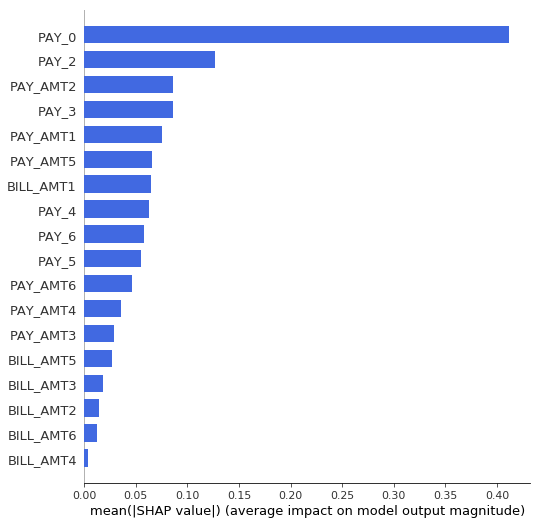
\includegraphics[height=1.17\linewidth, width=1.05\linewidth]{img/global_shap.png}
  		\caption{Consistent global Shapley feature importance values for $g_{\text{GBM}}$.}
  		\label{fig:global_shap}
	\end{subfigure}\hspace{10pt}
	\begin{subfigure}{.5\textwidth}
		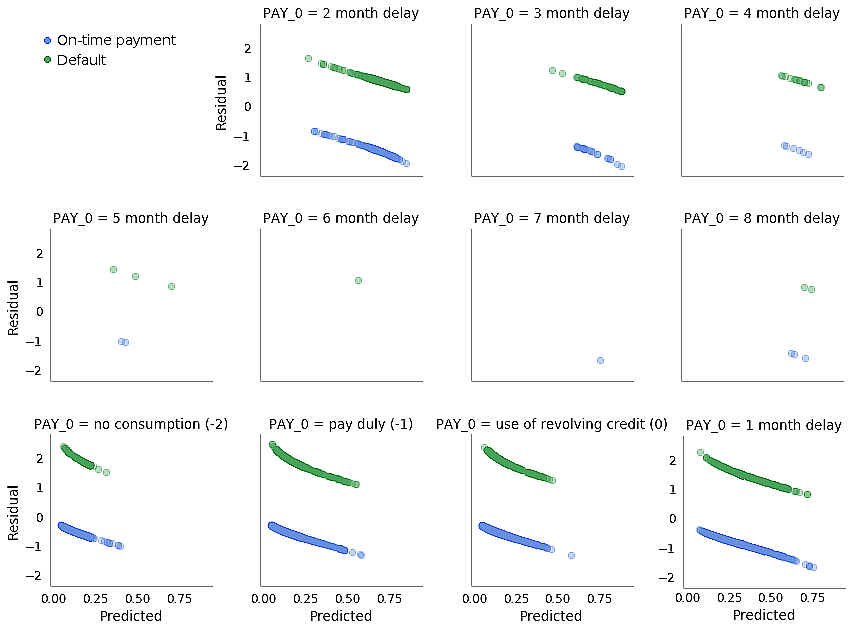
\includegraphics[width=1.2\linewidth]{img/resid.png}
  		\caption{$g_{\text{GBM}}$ deviance residuals and predictions by \texttt{PAY\_0}.}
  		\label{fig:resid}
	\end{subfigure}
	\caption{An unconstrained GBM probability of default model, $g_{\text{GBM}}$, over-emphasizes the importance of the input feature \texttt{PAY\_0}, a customer's most recent repayment status. $g_{\text{GBM}}$ produces large positive residuals when \texttt{PAY\_0} indicates on-time payments (\texttt{PAY\_0} $\leq$ 1) and large negative residuals when \texttt{PAY\_0} indicates late payments (\texttt{PAY\_0} $>$ 1). $g_{\text{GBM}}$ is explainable, but probably not trustworthy.}
	\label{fig:global_shap_resid}
\end{figure}

\item \textbf{Trust without explanation and understanding}: Years before reliable explanation techniques were widely acknowledged and available, black-box predictive models, such as autoencoder and MLP neural networks, were used for fraud detection in the financial services industry \cite{gopinathan1998fraud}. When these models performed well, they were trusted.\footnote{For example: \url{https://www.sas.com/en_ph/customers/hsbc.html}, \url{https://www.kdnuggets.com/2011/03/sas-patent-fraud-detection.html}.} However, they were not explainable or well-understood by contemporary standards.  

\end{itemize}

If trust in models is your goal, then explanations alone are not sufficient. However, as discussed in Section \ref{sec:white_box} and illustrated in Figure \ref{fig:hc_ml}, in an ideal scenario, explanation techniques would be used with a wide variety of other methods to increase accuracy, fairness, interpretability, privacy, security, and trust in ML models. 

\section{Guideline: Always Use Transparent ML Mechanisms for Systems That Affect Humans.}

Explainable ML tools like surrogate models, partial dependence plots, and global feature importance are already used to document, understand, and validate different types of models in the financial services industry \cite{lime-sup}, \cite{wf_xnn}.\footnote{Working paper: ``SR 11-7, Validation and Machine Learning Models, Tony Yang, CFA, CPA, FRM. KPMG USA.} Furthermore, adverse action notices are mandated under the Equal Credit Opportunity Act (ECOA) and the Fair Credit Reporting Act (FCRA) for many credit lending, employment, and insurance decisions in the United States.\footnote{See: \url{https://consumercomplianceoutlook.org/2013/second-quarter/adverse-action-notice-requirements-under-ecoa-fcra/}.} If machine learning is used for such decisions it must be explained in terms of adverse action notices.\footnote{This is apparently \textit{already} happening: \url{https://www.prnewswire.com/news-releases/new-patent-pending-technology-from-equifax-enables-configurable-ai-models-300701153.html}.} Shapley values, and other local feature importance approaches, provide a convenient methodology to rank the direct contribution of input features to final model decisions and potentially generate customer-specific adverse action notices. In a number of other application domains, broader interpretability is also legal necessity. Explanation, along with white-box models, model debugging, disparate impact analysis, and the documentation they enable, can also be required under the Civil Rights Acts of 1964 and 1991, the Americans with Disabilities Act, the Genetic Information Nondiscrimination Act, the Health Insurance Portability and Accountability Act, the Fair Housing Act, Federal Reserve SR 11-7, the European Union (EU) Greater Data Privacy Regulation (GDPR) Article 22, and other regulatory statutes \cite{ff_interpretability}.\\

Aside from regulatory mandates, explanation enables logical appeal processes for automated decisions made by ML models. Consider being negatively impacted by an erroneous black-box model decision, say for instance being mistakenly denied a loan or parole. How would you argue your case for appeal without knowing how model decisions were made? According the New York Times, a man named Glenn Rodr\'iguez found himself in this unfortunate position in Upstate New York in 2016.\footnote{This too is happening \textit{today}: \url{https://www.nytimes.com/2017/06/13/opinion/how-computers-are-harming-criminal-justice.html}.}\\

Some may argue that, outside of regulated dealings, for a model with little or no impact on humans and that has been thoroughly and responsibly tested by knowledgeable practitioners, that explanation is \textit{really} unnecessary. While that statement appears technically true, the counter argument in this case centers on human learning from ML models. Explanatory techniques allow us to gain insights from complex models about nonlinear phenomena and complex interactions -- information that may sometimes be unlearnable by linear models. Why go through the weeks, months, or years of training and deploying a production ML system, and not take a small percentage of that time to learn about the model's findings?\\ 


\section{Guideline: Use Direct XAI Techniques in Addition to Surrogate Models Whenever Possible.}

Models of models, or surrogate models, can be helpful explanatory tools, but they are usually approximate, low-fidelity explainers. Aside from 1.) a global summary of a complex model provided by a surrogate model can be helpful sometimes and 2.) much work in explainable ML has been directed toward improving the fidelity and usefulness of surrogate models \cite{dt_surrogate2}, \cite{viper}, \cite{dt_surrogate1}, \cite{lime-sup}, \cite{wf_xnn}, \textbf{many explainable ML techniques have nothing to do with surrogate models!} One of the most exciting breakthroughs for supervised learning problems in explainable ML is the application of a coalitional game theory concept, Shapley values, to compute feature contributions which are consistent globally and accurate locally using the trained model itself \cite{shapley}, \cite{kononenko2010efficient}. An extension of this idea, called tree SHAP, has already been implemented for popular tree ensemble methods \cite{tree_shap}. 

\begin{figure}[htb!]
	\begin{subfigure}{.55\textwidth}
		\includegraphics[height=0.6\linewidth, width=.95\linewidth]{img/dt_surrogate.png}
  		\caption{Na\"ive $h_{\text{tree}}$, \textit{a surrogate model}, forms an approximate overall flowchart for the explained model, $g_{\text{GBM}}$.}
  		\label{fig:dt_surrogate}
	\end{subfigure}\hspace{5pt}
	\begin{subfigure}{.45\textwidth}
  		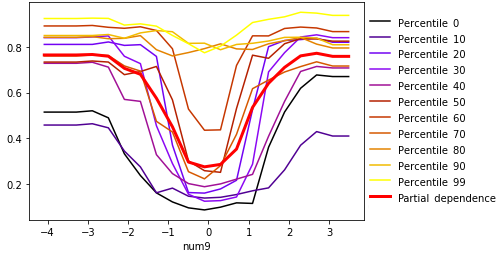
\includegraphics[height=.52\linewidth, width=1.02\linewidth]{img/pdp_ice.png}
  		\caption{Partial dependence and ICE curves generated \textit{directly from the explained model}, $g_{\text{GBM}}$.}
  		\label{fig:pdp_ice}
	\end{subfigure}
	\caption{$h_{\text{tree}}$ displays known interactions in $f = X_{\text{num}1} * X_{\text{num}4} + |X_{\text{num}8}| * X_{\text{num}9}^2$ for $\sim -0.923 < X_{\text{num9}} <  \sim 1.04$. Modeling of the known interaction between $X_{\text{num9}}$ and $X_{\text{num8}}$ in $f$ by $g_{\text{GBM}}$ is confirmed by the divergence of partial dependence and ICE curves for $\sim -1 < X_{\text{num9}} <  \sim 1$. Explanations from a surrogate model have augmented and confirmed findings from a direct model visualization technique.}
	\label{fig:pdp_ice_dt_surrogate}
\end{figure}

There are many other explainable ML methods that operate on trained models directly such as partial dependence, ALE, and ICE plots \cite{ale_plot}, \cite{esl}, \cite{ice_plots}. Surrogate models and explanatory techniques that operate directly on trained models can also be combined, for instance by using partial dependence, ICE, and surrogate decision trees to investigate and confirm modeled interactions \cite{art_and_sci}. In Figure \ref{fig:pdp_ice_dt_surrogate}, an unconstrained GBM, $g_{\text{GBM}}$, models a known signal generating function $f$:

\begin{equation}
\label{eq:f}
f(\mathbf{X}) = \twopartdef {1} {X_{\text{num}1} * X_{\text{num}4} + |X_{\text{num}8}| * X_{\text{num}9}^2 + e \geq 0.42} {0} {X_{\text{num}1} * X_{\text{num}4} + |X_{\text{num}8}| * X_{\text{num}9}^2 + e < 0.42}
\end{equation}

\noindent where $e$ signifies the injection of random noise in the form of label switching for roughly 15\% of the training and validation observations.\footnote{Code to replicate Figure \ref{fig:pdp_ice_dt_surrogate} is available here: \url{https://github.com/h2oai/mli-resources/tree/master/lime_shap_treeint_compare}.} $g_{\text{GBM}}$ is then trained such that $g_{\text{GBM}}(\mathbf{X}) \approx f(\mathbf{X})$ in training and validation data. $h_{\text{tree}}$, displayed in Figure \ref{fig:dt_surrogate}, is extracted such that $h_{\text{tree}}(\mathbf{X}) \approx g_{\text{GBM}}(\mathbf{X}) \approx f(\mathbf{X})$ in validation data. Partial dependence and ICE plots are generated directly for $g_{\text{GBM}}$ in the same validation data and overlaid in Figure \ref{fig:pdp_ice}. The parent-child node relationship displayed between $X_{\text{num9}}$ and $X_{\text{num8}}$ for $\sim -0.923 < X_{\text{num9}} <  \sim 1.04$ in \ref{fig:dt_surrogate} and the divergence of ICE and partial dependence curves in \ref{fig:pdp_ice} for $\sim -1 < X_{\text{num9}} <  \sim 1$ help confirm and understand how $g_{\text{GBM}}$ learned the interaction between $X_{\text{num}8}$ and $X_{\text{num}9}$ in $f$. Like in Figure \ref{fig:global_shap_resid}, combining different approaches provided additional, beneficial information about a complex ML model.\\ %For a curated list of many other different types of white-box modeling techniques, and model-specific, model-agnostic, and surrogate model explainable ML techniques, please see:

%\begin{center}
%\url{https://github.com/jphall663/awesome-machine-learning-interpretability}
%\end{center}

\noindent\textbf{Guideline Corollary: Don't use LIME alone.} LIME is important, imperfect, and one of many explainable ML tools. LIME, in it's most popular implementation, uses local linear surrogate models to explain regions of complex, machine-learned response functions \cite{lime}. And again, LIME can sometimes be combined with model-specific methods to yield deeper insights. Consider that tree SHAP can provide locally accurate and consistent point estimates for local feature importance as in \ref{fig:shap}. LIME can then provide approximate information about modeled local linear trends around the same point. Table \ref{tab:lime} contains LIME $h_{\text{GLM}}$ coefficients for a local region of a validation set sampled from the UCI credit card data defined by \texttt{PAY\_0 > 1.5}, or customers with a fairly high risk of default due to late most recent payments.\footnote{Code to replicate Table \ref{tab:lime} is available here: \url{https://github.com/jphall663/xai_misconceptions}.} $h_{\text{GLM}}$ models the predictions of a simple interpretable decision tree model, $g_{\text{tree}}$, displayed in \ref{fig:dt}. $h_{\text{GLM}}$ coefficients show linear trends between features in the sampled set $\mathbf{X}_{\text{PAY\_0} > 1.5}$ and $g_{\text{tree}}(\mathbf{X}_{\text{PAY\_0}> 1.5})$. Because $h_{GLM}$ is relatively well-fit (0.73 $R^2$) and has a logical intercept (0.77), it can be used along with Shapley values to reason about the modeled average behavior for risky customers and to differentiate the behavior of any one specific risky customer from their peers under the model. This additional information can be useful for model validation and compliance purposes.

\begin{table}[htb!]
	\caption{Coefficients for a local linear interpretable model, $h_{\text{GLM}}$, with an intercept of 0.77 and an $R^2$ of 0.73. $h_{\text{GLM}}$ is trained on a segment of the UCI credit card dataset containing higher-risk customers with late most recent repayment statuses, $\mathbf{X}_{PAY \_ 0 > 1.5}$, and the predictions of simple decision tree, $g_{\text{tree}}(\mathbf{X}_{\text{PAY\_0} > 1.5})$.}
		\centering
			%\tiny
				\begin{tabular}{ | p{2cm} | p{1.7cm} | }
				\hline
				$h_{\text{GLM}}$\newline Feature & $h_{\text{GLM}}$\newline Coefficient \\ 
				\hline
				\texttt{PAY\_0 == 4} & $0.0009$ \\
				\hline
				\texttt{PAY\_2 == 3} & $0.0065$ \\
				\hline
				\texttt{PAY\_5 == 2} & $-0.0006$ \\
				\hline
				\texttt{PAY\_6 == 2} & $0.0036$ \\
				\hline				
				\texttt{BILL\_AMT1} & $3.4339\mathrm{e}{-08}$ \\
				\hline
				\texttt{PAY\_AMT1} & $4.8062\mathrm{e}{-07}$ \\
				\hline	
				\texttt{PAY\_AMT3} & $3.4338\mathrm{e}{-08}$ \\	
				\hline	
			\end{tabular}	
  		\label{tab:lime}
\end{table}	

\section{Guideline: Understand How XAI Can Be Used for Nefarious Purposes.}

If used disingenuously, explainable ML methods can provide cover for misused or intentionally abusive black-boxes \cite{fair_washing}. But explainable ML methods were designed specifically to crack open those same nefarious and complex black-boxes. See Angwin et al. (2016) for evidence that hacking or stealing of commercial black-box models for oversight purposes is possible \cite{angwin16}.\footnote{This text makes no claim on the quality of the analysis in Angwin et al. (2016), which has been criticized \cite{flores2016false}. This now infamous analysis is presented only as evidence that motivated activists can hack or steal commercial black-boxes.} Such investigations would likely only be improved by advances in explanatory and fairness tools. Additionally, many important computer-based technological advances present similar double-edged sword dilemmas, e.g. social media or strong encryption. Rarely does the ability of a tool to be misused for malicious purposes disqualify it from being used as designed. Given that explainable ML techniques have already been released in popular open source software, it seems there is a need for agreed-upon best practices and education on responsible use.  


\section{Guideline: Use XAI Techniques Along with Interpretable Models for Systems That Affect Humans.}\label{sec:white_box}

\begin{figure}[ht!]
	\begin{subfigure}{.6\textwidth}
		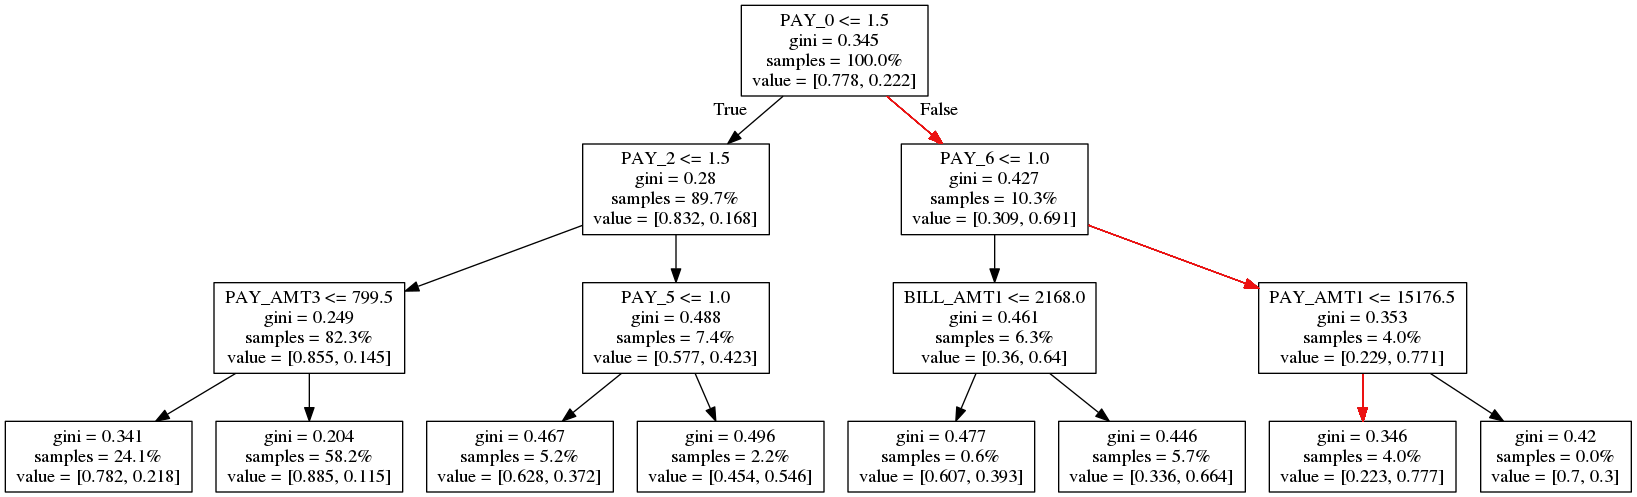
\includegraphics[height=.45\linewidth, width=1.15\linewidth]{img/dt.png}
  		\caption{Simple decision tree, $g_{\text{tree}}$, trained on the UCI credit card data to predict default with validation AUC of 0.74. The decision policy for a high-risk individual is highlighted in red.}
  		\label{fig:dt}
	\end{subfigure}\hspace{50pt}
	\begin{subfigure}{.4\textwidth}
		\vspace{30pt}
  		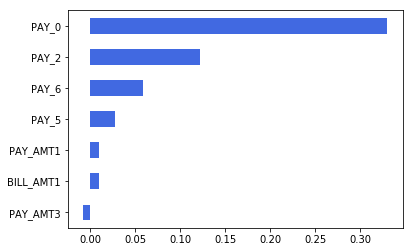
\includegraphics[height=.5\linewidth, width=.8\linewidth]{img/shap.png}
  		\vspace{5pt}
  		\caption{Locally-accurate Shapley contributions\\ for the highlighted individual's probability\\ of default.}
  		\label{fig:shap}
	\end{subfigure}
	\caption{}
	\label{fig:dt_shap}
\end{figure}

A few well-known publications have focused either on white-box modeling techniques (e.g. \cite{slim}, \cite{sbrl}) or on post-hoc explanations (e.g.  \cite{shapley}, \cite{lime}), but the two can be used together in the context of a broader and more human-centered machine learning workflow as illustrated in Figure \ref{fig:hc_ml}. Consider the seemingly useful example case of augmenting globally interpretable models with local post-hoc explanations. A practitioner could train a single decision tree, a globally interpretable model, then apply local explanations in the form of Shapley feature importance as illustrated in Figure \ref{fig:dt_shap}.\footnote{Code to replicate Figure \ref{fig:dt_shap} is available here: \url{https://github.com/jphall663/xai_misconceptions.}} This enables the practitioner to see accurate numeric feature contributions for each model prediction in addition to the entire directed graph of the decision tree. Even for interpretable models, such as linear models and decision trees, it has been shown that Shapley values present accuracy and consistency advantages over standard feature attribution methods \cite{lipovetsky2001analysis}, \cite{tree_shap}, \cite{shapley}. In Figure \ref{fig:dt_shap}, a simple decision tree, $g_{\text{tree}}$, is trained on the UCI credit card data set to predict probability of default. $g_{\text{tree}}$ has a validation AUC of 0.74. The decision-policy for a high-risk customer is highlighted in \ref{fig:dt} and the locally-accurate Shapley contributions for this same individual's predicted probability are displayed in \ref{fig:shap}. The Shapley values are helpful because they highlight the local importance of \texttt{PAY\_2}, the individual's second most recent repayment status, which could be underestimated by examing the decision policy alone. The Shapley values also enable the ranking of input features for each model decision, which is likely helpful for FCRA and ECOA compliance. Another twist on the idea of combining explainable AI methods and white-box models is described in ``Surrogate Assisted Feature Extraction for Machine Learning (SAFE ML)'' \cite{gosiewska2019safe}. In the SAFE ML approach, features learned by more complex models are extracted and used in an explainable fashion to increase the accuracy of more interpretable models. Aren't either of these augmented processes more desirable than either a white-box model or post-hoc explanations alone?\\ 

\noindent\textbf{Guideline Corollary: Use Explainable ML Methods with Disparate Impact Analysis.} Like white-box models, fairness methods (e.g. \cite{feldman2015certifying}, \cite{hardt2016equality}) are often presented in different articles than post-hoc explanatory methods. However, in banks, using post-hoc explanatory tools such as partial dependence plots to comply with model documentation guidance often goes hand-in-hand with using disparate impact analysis to comply with fair lending regulations.\footnote{Working paper: “SR 11-7, Validation and Machine Learning Models”. Tony Yang, CFA, CPA, FRM. KPMG USA.}\textsuperscript{,}\footnote{White paper: \url{https://www.aba.com/Compliance/Documents/FairLendingWhitePaper2017Apr.pdf}}\textsuperscript{,}\footnote{Policy Statement on Discrimination in Lending: \url{https://www.govinfo.gov/content/pkg/FR-1994-04-15/html/94-9214.htm}} 

\begin{table}[htb!]
	\centering
	\caption{Basic group disparity metrics across different marital statuses for monotonically constrained GBM model, $g_{\text{mono}}$, trained on the UCI credit card dataset.} 
	\footnotesize
	\begin{tabular}{ | p{1.1cm} | p{1.1cm} | p{1.3cm} | p{1.2cm}| p{1.2cm} | p{1.2cm} | p{1.2cm} | p{1.2cm} | }
	\hline
	& Adverse\newline Impact\newline Disparity & Accuracy Disparity & TPR\newline Disparity & TNR\newline Disparity & FPR\newline Disparity & FNR\newline Disparity \\ 
	\hline
	\texttt{married} & 1.00 & 1 .00 & 1.00 & 1.00 & 1.00 & 1.00 \\
	\hline	
	\texttt{single} & 0.89 & 1.03 & 0.99 & 1.03 & 0.85 & 1.01 \\
	\hline	
	\texttt{divorced} & 1.01 & 0.93 & 0.81 & 0.96 & \textcolor{red}{1.25} & 1.22 \\
	\hline
	\texttt{other} & \textcolor{red}{0.26} & 1.12 & \textcolor{red}{0.62} & 1.17 & \textcolor{red}{0} & \textcolor{red}{1.44} \\
	\hline	
	\end{tabular}
	\label{tab:dia}
\end{table}

Table \ref{tab:dia} displays basic group parity metrics for a monotonically constrained GBM model, $g_{\text{mono}}$, trained on the UCI credit card data.\footnote{Code to replicate Table \ref{tab:dia} is available here: \url{https://github.com/jphall663/xai_misconceptions}.} In this example scenario, $g_{\text{mono}}$ displays group parity according to the four-fifths rule with \texttt{married} as the reference level for single customers, but exposes potential disparate impact for \texttt{divorced} customers and customers with martial status of \texttt{other} (for which there is very little training data).

\section*{Conclusion}

Machine learning systems are used today to make life-altering decisions about employment, bail, parole, and lending.\footnote{ICLR 2019 model debugging workshop CFP: \url{https://debug-ml-iclr2019.github.io/}} The scope of decisions delegated to machine learning systems seems likely only to expand in the future. Many researchers and practitioners are tackling disparate impact, inaccuracy, privacy violations, and security vulnerabilities with a number of brilliant, but perhaps siloed, approaches. By addressing some common explainable ML misconceptions, this short text also gives examples of combining innovations from several sub-disciplines of machine learning research to train explainable, fair, and trustable predictive modeling systems. As proposed in Figure \ref{fig:hc_ml}, using these techniques together can create a new and more human-centered type of machine learning potentially suitable for use in business- and life-critical decision support.\\

\vspace{100pt}

\begin{figure}[htb!]
	\begin{center}
		\includegraphics[scale=0.15]{img/hc_ml.png}
		\caption{A diagram of a proposed human-centered machine learning workflow in which explanations (highlighted in green) are used along with interpretable models, disparate impact analysis and remediation techniques, and other review and appeal mechanisms to create a fair, accountable, and transparent ML system.}
		\label{fig:hc_ml}
	\end{center}
\end{figure}

\section*{Acknowledgemnts}

The author thanks Przemyslaw Biecek, Pramit Choudhary, Navdeep Gill, and Christoph Molnar for their helpful input and insights. 

%-------------------------------------------------------------------------------
\section*{References}
%-------------------------------------------------------------------------------
\small
\bibliographystyle{plain}
\bibliography{responsible_xai}

\end{document}

% let doug proofread